% This is sigproc-sp.tex -FILE FOR V2.6SP OF ACM_PROC_ARTICLE-SP.CLS
% OCTOBER 2002
%
% It is an example file showing how to use the 'acm_proc_article-sp.cls' V2.6SP
% LaTeX2e document class file for Conference Proceedings submissions.
% ----------------------------------------------------------------------------------------------------------------
% This .tex file (and associated .cls V2.6SP) *DOES NOT* produce:
%       1) The Permission Statement
%       2) The Conference (location) Info information
%       3) The Copyright Line with ACM data
%       4) Page numbering
%
%  However, both the CopyrightYear (default to 2002) and the ACM Copyright Data
% (default to X-XXXXX-XX-X/XX/XX) can still be over-ridden by whatever the author
% inserts into the source .tex file.
% e.g.
% \CopyrightYear{2003} will cause 2003 to appear in the copyright line.
% \crdata{0-12345-67-8/90/12} will cause 0-12345-67-8/90/12 to appear in the copyright line.
%
% ---------------------------------------------------------------------------------------------------------------
% It is an example which *does* use the .bib file (from which the .bbl file
% is produced).
% REMEMBER HOWEVER: After having produced the .bbl file,
% and prior to final submission,
% you need to 'insert'  your .bbl file into your source .tex file so as to provide
% ONE 'self-contained' source file.
%
% Questions regarding SIGS should be sent to
% Adrienne Griscti ---> griscti@acm.org
%
% Questions/suggestions regarding the guidelines, .tex and .cls files, etc. to
% Gerald Murray ---> murray@acm.org
%
% For tracking purposes - this is V2.6SP - OCTOBER 2002

\documentclass{acm_proc_article-sp-sigmod07}
\usepackage{graphicx}
\usepackage{hyperref}
\begin{document}
%
% --- Author Metadata here ---
%\conferenceinfo{ACM SIGMOD}{'07 Beijing, China}
%\setpagenumber{50}
%\CopyrightYear{2002} % Allows default copyright year (2002) to be over-ridden - IF NEED BE.
%\crdata{0-12345-67-8/90/01}  % Allows default copyright data (X-XXXXX-XX-X/XX/XX) to be over-ridden.
% --- End of Author Metadata ---

\title{A new massive data analytics approach to the football}
%
% You need the command \numberofauthors to handle the "boxing"
% and alignment of the authors under the title, and to add
% a section for authors number 4 through n.

\author{Marco De Nadai, Michele Linardi}
%
\maketitle
\begin{abstract}
This paper approaches the football similarly to what Moneyball has made in US baseball. This work wants to create a small framework of tools which permits the coaches to base their new strategies not only on their intuitions and judgments but also on comprensive (and maybe not human-eye-visible) statistics. Using the past researches in the football and sport fields, it will analyze a match recorded by DEBS with an innovative system of sensors which could be the future of football. 
\end{abstract}



\section{Introduction}
In a modern (or post-modern) society where the hero-cult, self-improvements and the game are important, and where the multi-etnics/culturality are increasing, the sport influence is uncontested \cite{pelivs2003sport}.
Football is the most popular sport in the world but, while the national and international competition increases, the investments need to diminish due to the high debts reached from all the major football clubs (only in the italian Serie A there are 1.6B euro of debts \cite{gazzetta}]). It is clear that without new money and investments, it is not possible to follow the self-serving megalomania \cite{progression}, which conducted these clubs to this point. They need to rely in alternative system.\\
This situation is very similar to what the Okland Athletics' general manager, Billy Beane faced in 2002: Okland Athletics (OA) was in an unfavourable financial situation after 2001 postseason. For this reason, he focused his attention on the team’s analytical, evidence-based SABS \cite{grabiner1999sabermetric}, approach to assemble a competitive team which challenged teams such as the New York Yankees, who spent three times more than OA in payroll that same season. His approach, well described in the book \emph{Moneyball, the art of winning an unfair game}, was based in tricky stats which contributed in the selection of player who could have leaded to the World series victory. Bill James condensed the SABS' reasoning on this quote: "sabermetrics attempts to answer objective questions about baseball, such as "which player on the Red Sox contributed the most to the team's offense?" or "How many home runs will Ken Griffey hit next year?" It cannot deal with the subjective judgments which are also important to the game, such as "Who is your favorite player?" or "That was a great game." \cite{grabiner1999sabermetric}.

After a utopic OA season, Moneyball has made an undeniable impact in the baseball major league, hence the most important teams have hired full-time SABS analysts and have started to follow its principles. Although football is related to his "stop and go" nature, in 2009 \emph{Soccernomics} approached the European football as Moneyball did for U.S. baseball, influencing the selection of players in a team.
However, the other reason to analyse players is linked to the exploitation of the factors, which contribute to optimal players' performances: examining these factors, coaches could understand camouflaged problems and train better the players. They could analyse a match to identify the major team's strengths, which can be further developed, or its major weaknesses, which suggest areas for improvement. Similarly, the same analysis applied to the opposite team, could make the strategy development easier to the coach \cite{lago2010game}. The increased research activity in this field has been particular evident in soccer, where the importance of scientific research has became increasingly accepted \cite{ScienceSoccer}.

The player monitoring during a competition were originally achieved using manual video-based motion analysis, but the perceived complexity and time consumption formed barriers to its adoption \cite{james2006role}. In the last decade, teams often used automatic motion analysis realized with system based on PITCHf/x with many limits, errors, problems \cite{Choi20111274}\cite{Figueroa2006122} which did not lead to meaningful results and consequently did not justify they high maintaining costs.\\
The recent 2013 MIT Sloan sport analytics conference emerged \cite{mitsloan} the rise of spatial data, which are extremely important in every sports to explain trickily problems inside a team with a high accuracy. The use these wireless GPS systems to track players movements during a match, connected with high quality data visualization makes complex data analysis interesting, useful and understandable to GM and business people. The intense competitive schedules of elite soccer clubs require data to be available usually within 24-36 hours post-match \cite{Figueroa2006122}, for this reason we decided to use the DEBS 2013 conference \cite{debs2013} challenge \cite{debs20131} dataset to analyse a football match and the players involved. We will use the recent data mining technologies in order to exploit different meaningful tools to the coaches.

\section{Related works}
When Bill James and SABR-metrician were making their contributions to baseball, they worked in public data. Nowadays things are different: sport analytics is made primarily in-house, were number crunchers can work secretly in order to gain a competitive advantage. This peculiarity is true especially in football, where companies like Opta in England, Adidas in USA and many others (Sport/VU, Prozone etc) are contracted to gather in depth stats to the teams who do not distribute their dataset. Despite that, there are some exception like Manchester City FC, who made available to the world the MCFC Anaytics project: some statistical data on the 2011-12 English Premier League.

\section{Proposed approach}
The importance of teams is widely accepted \cite{Wisdom}\cite{vancollaboration} and the right composition of teams determines their odds or success \cite{guimera2005team}\cite{wuchty2007increasing}. The difficulty relies in the understanding what and who is important in a team.\\
Football analysis is not easy as baseball; indeed the first is a unique sport, characterized by continuous, cooperative and interdependent actions, hybrid offensive and defensive roles and thousands of thousands of variables dependents from the team’s strategy. This makes very difficult to exploit what is important in a match in order to achieve a victory and forces researchers to analyse many matches and tournaments in order to discover similar patterns.
 
The easier statistic adopted in the past has been the possession percentage; to cite Johan Cruijff: "As long as we have got the ball, they can't score". However, this metric is gradually losing ground as the recent researcher states \cite{newyorkredbulls}. In the researches so far, efficient attacks were analysed in the European Championships, World competitions/championships, high quality club competitions but these studies' outcome are contradictory. Indeed for example, if talk again about possession, Hook and Hughes (2001) found that successful teams utilised longer possession than unsuccessful teams in Euro 2000; instead in a similar study Stanhope (2001) found that time in possession of the ball was not indicative of success in the 1994 World Cup. Other studies have tried to provide a "formula" of winning but anyone came out with a definitive conclusion \cite{lago2010game}. Nonetheless, the latest research in this field focuses in the network analysis to study the relations of players in the matches, as a system biology group explained 	\cite{duch2010quantifying}. Hence, we concluded that a "final formula" does not exist and statistics needs to be helpful to coaches and not a substitute to them. For this reason we will analyse four different characteristics from the DEBS challenge: similar players to train, passages patterns, clustering of trajectories and apeed perfornance analysis.

\subsection{The dataset}
The purpose of this work is exploiting some useful hidden informations of a football match, using the data recorded by the sensor provided by Fraunhofer, used in the challenge promoted by the \cite{debs2013} conference. This dataset is composed by a set of positions of players and balls which records the activity of a soccer match.

The event schema of the sensor recording is following: \texttt{sid, ts, x, y, z, |v|, |a|, vx, vy, vz, ax, ay, az} where \texttt{sid} is a sensor id which produced the position event, \texttt{ts} is a timestamp in picoseconds, e.g.: 10753295594424116 (\texttt{x}, \texttt{y}, \texttt{z} describe the position of the sensor in mm (the origin is the middle of a full size football field) ; \texttt{|v|} (in μm/s), \texttt{vx}, \texttt{vy}, \texttt{vz} describe direction by a vector with size of 10,000. \texttt{ax}, \texttt{ay}, \texttt{az} describe the absolute acceleration and its constituents in three dimensions (the acceleration in $m/s^2$ is calculated similar to that of the velocity). The acceleration does not include gravity, i.e. \texttt{|a|} is zero when the ball is at a fixed position and not $9.81 m/s^2$). 

\subsection{Similar players to train}
Past research focuses \cite{lago2010game} concluded that the variables that better differentiate winning, losing and drawing teams in a global way were the following: total shots, shots on goal, crosses, crosses against, ball possession and venue (fixed in our dataset). Despite that it seems clear that the ability to retain possession of the ball is linked to success, we will not consider the possession time due to the problems described before; we will only consider the players' effectiveness.
Moreover it is also proved that the second half of the match is significantly more efficient and the efficient attacks are initiated mostly by interception of opponents' passes 	\cite{jankovic}, so we counted the tackles, weighting them considering the first/second half of the match.
All the weights are based on the multivariate test of \cite{lago2010game}, and it conduct to a multi-dimensional value which summarizes the player quality. Afterthat we will group the players into similar clusters. 

Our Python code reads the whole dataset with the csv reader/writer module, which permits a good organization and balance between the memory and I/O used. In the code we start excluding every sensors which are out from the field, afterthat we observe either the ball and the players. Some game considerations/euristics are necessary:
\begin{itemize}
  \item A ball is hit if it reaches the minimal acceleration of $55 m/s^2$
  \item A player possess the ball if the distance from one of his foot (transmitter) is less than 1 meter and he keeps it in a time between 0.2 seconds and 1 second.
  \item The ball is crossed if the z-coordinate is greater than 2 meters.
  \item There is a tackle if the team possession changes in a short time and between two players sensors within 2 meters of distance.
\end{itemize}
The code analyses some dimensions obtained by different different reasearches in the football field. Consequently the analyzed metrics are:
\begin{description}
  \item[successful/unsuccessful passages] important for the ability to retain possession of the ball, linked to the effectiness of attack/defense
  \item[unsuccessful passages on defensive third] dangerous errors near the goal
  \item[successful/unsuccessful crosses] important actions for an effective attack \cite{lago2010game}
\item[total shots and shots on goal] important actions for an effective attack \cite{lago2010game}
\item[won/lost tackles] important for the interceptions and the consequently construction of the actions, especially in the second half of the match \cite{jankovic}
\end{description}

Afterthat, the code will save the results into a transition SQLite database which can be used many times with different algorithms and parameters without lunching the analyzation again.

The second part of the work is addressed to give mean to the numbers, clustering the similar players into groups and attaining high intra-cluster similarity (documents within a cluster are similar) and low inter-cluster similarity (documents from different clusters are dissimilar).\\
A number of clustering algorithms with different characteristics has been reported in literature, hence we examinated a considerable number of them, including hierarchical and partition clustering algorithms. The first group seeks to build nested clusters by merging them successively. It is divided in two main categories: agglomerative and divide. They are very useful for our project because they use a distance matrix to compare the similar object in a set and they need only a termination condition. Partition-based clustering algorithms' aim is to partition the observations into k clusters in which each observation belongs to the cluster with nearest mean.

The hierarchy-clustering algorithm selected is Ward which is a variance-minimizing agglomerative clustering. The purpose of this algorithm is to unify groups such that the variation inside them does not increase too drastically. Specifically it joins the groups that give the smallest increase in:
$$\Delta(P,Q) = {n_Pn_Q \over n_P+n_Q} d^2(P,Q)$$
This procedure will make clusters as homogeneous as possible. This type of clustering is used in our work in order to visually plot a dendogram, which specify the similarity of the groups. Coaches could form groups or think about strategies visually.

The partition based clustering algorithm we will use is K-means \cite{forgy1965cluster}, which requires the k number of clusters we want in output. It starts identifying k cluster centers and then it calculates the distances of observations from the k-centers and assigns each observation to the nearest center, forming a group. After that it calculates the new center of each group and start again to assign the observations to the nearest cluster center. The procedure stabilizes when none of the N objects changes the membership.  The major weaknesses of this algorithm are not significant to our work:
\begin{itemize}
  \item the number of clusters, which needs to given in advance could be the number of available coaches of a team. For example if one club has three coaches, it could train its players grouping them by similarity. This could make the workout very efficient.
  \item Its sensitivity to noisy data and outliers is not a problem because we need to train every team’s player: no one could avoid the workout.
\end{itemize}
As mentioned above, the algorithm needs to locate the first k centers and it could be done randomly. We will use instead the k-means++ heuristic \cite{arthur2007k}, which iteratively chooses the next seed with probability depending on how far apart it is from any of the currently selected seeds.\\
The result of k-means clustering is composed by the k-clusters of players and the mean of their weaknesses, useful to address the training.

\begin{figure}
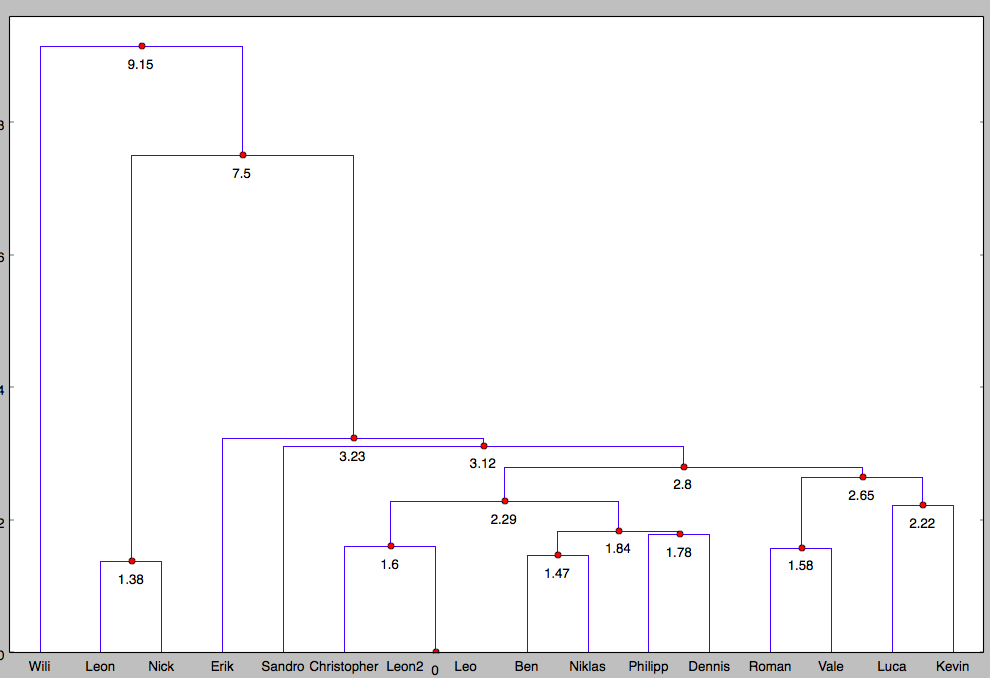
\includegraphics[scale=0.24]{arg}
\caption{Dendogram of the hierarchical clustering}
\end{figure}

\subsection{Passages patterns}
This work is based on the methodology created by a group of system biology, which studied the importance of players, and those passes in the Euro 2008 tournament \cite{duch2010quantifying}. In order to measure the player importance in a team, each player is represented in a graph with a node and the passages between the different players with an edge. The darker the node colour is, the more efficiency he reached. Similarly the thicker the edge is the more number of passages he did with the linked player. This result is strongly connected to the previous tool we developed and we refer to it for further explanations. \\
The output graph could be used by coaches to valuate the importance of players (and superstar-players) into their team. Similarly it can be use to build a strategy for an incoming match.

\begin{figure}
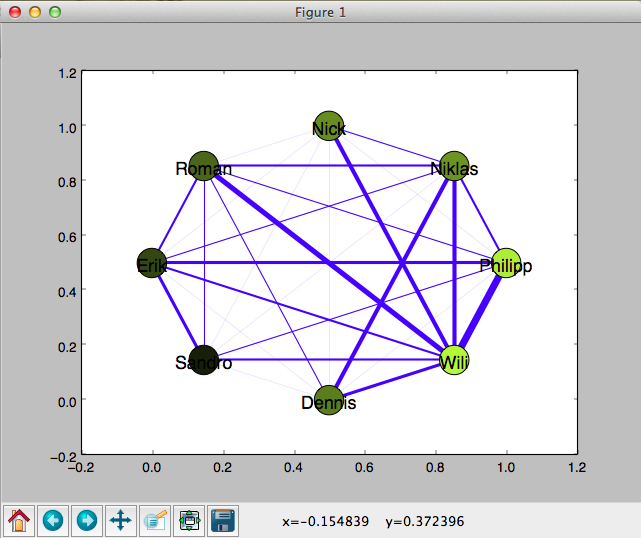
\includegraphics[scale=0.38]{edge}
\caption{Passages patterns of team 1}
\end{figure}

\subsection{Clustering of trajectories}
In order to make good strategies the soccer coaches analyze the archives of matches. Since the soccer is a very complicated game due to a large number of participants for each team and for the several types of existing roles, in our opinion, understand the dynamic of the movement of a single player could be meaningful for several problems. First of all discover the recurrent patterns of a player movements is useful to understand how the player usually act and this can reveal two several important things:
\begin{enumerate}
  \item Discover if a player is compatible with a module or with the type of play that the coach wants to adopt. 
  \item Discover if two or more player have the same movements.
  \item Understand the movement of a striker in order to apply the best defensive strategy, and of course the symmetric problem (understand how the defenders move to discover the portion of field where develop the action).
\end{enumerate}
In order to formalize this problem we can state the follow main points:
\begin{enumerate}
  \item Find the set of all significant trajectories for each player
  \item Find the set of all significant trajectories for the ball
  \item Cluster (group) all the similar trajectory of a single player or the similar trajectory of two or more player. In the same fashion, we will cluster the entire trajectory for the ball.
\end{enumerate}

\subsubsection{Find the meaningful trajectory}
Now we can define the first point related to the discovery of significant trajectory of players and we will show how we extract them in real time from the sensor data.
The first extraction from the data aims to store the trajectory, recording the single point of the player every second (we assume reasonable to log the movement of the player with this frequency). At the end of this step we have a sorted set of point $P = \{x_1, x_2, \ldots, x_n\}$ that tell us the activity of the player in the key moments of a match.\\
Now we can shift toward the second main problem that is to find the similar trajectory using an intuitive and powerful framework called TRACLUS \cite{lee2007trajectory}. The optimal partitioning of a trajectory should possess two desirable properties: preciseness and conciseness. Preciseness means that the difference between a trajectory and a set of its trajectory partitions should be as small as possible, conciseness means that the number of trajectory partitions should be as small as possible. In order to find the best set of characteristic point, in other words, the set of point where the trajectory has a significant change of behaviors the TRACLUS partitioning algorithm aims to find the best trade off between conciseness and preciseness. 


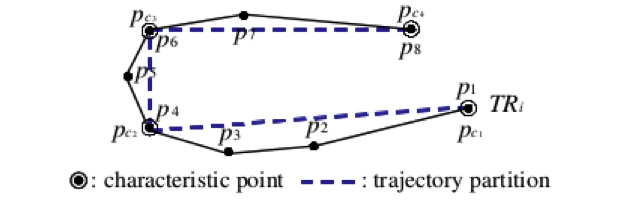
\includegraphics[scale=0.8]{traclus1}

The TRACLUS framework uses the MDL (Minimum description length) principle to minimize the trade off between conciseness and preciseness. Using this principle we have two values $L(H)$ that measure the degree of conciseness, and $L(D|H)$ that of preciseness. H is the hypothesis and it corresponds to a specific set of trajectory partitions and D the data thus the whole trajectory. 
$L(H)$ is the length, in bits, of the description of the hypothesis and $L(D|H)$ is the length, in bits, of the description of the data when encoded with the help of the hypothesis. $L(H)$ is computed summing the length of all the segment formed by the characteristic point. $L(D|H)$ is computed summing the difference between each segment with the whole trajectory.
The difference is computed with the help of three distances:
\begin{enumerate}
  \item Perpendicular distance
  \item Parallel distance
  \item Angle distance
\end{enumerate}
These distances are used for determining the trajectory similarity during the clustering process as well.
To compute $L(D|H)$ are used only the perpendicular and angle distance, the parallel distance is discard because the sub-trajectories belong to the same trajectory. 


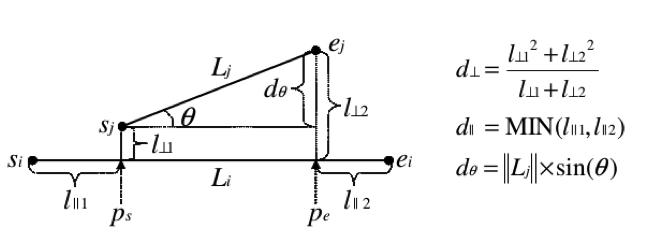
\includegraphics[scale=0.8]{traclus2}

At the end we keep the partition that minimize the summation: $L(H) + L(D|H)$.
We find that exploiting this method of partitioning we obtain a valid extraction of the meaningful trajectories of a player. We will see the experimental results that give us an important feedback about the quality of information gathered in the context of football.  \\
At the end of the partitioning as mentioned above we run the clustering algorithm that accept in input all the sub-trajectories partitioned that represent the interesting movement. 
As the major of the density-based cluster algorithm, also the TRACLUS suffers the problem of the parameter depending. Specifically there are two parameters to be set:
\begin{enumerate}
  \item Epsilon-Neighborhood, that permits to discovery the belongingness of a sub-trajectory to a specific cluster.
  \item MinLns, that is a parameter telling us the minimum size of the clusters and the number of the original trajectories where the sub-trajectories have to come from.
\end{enumerate}
Now we are going to describe how we solved the problem of the parameter discovery.
 
For the Epsilon-Neighborhood, we can exploit the method yield by the TRACLUS framework where it attempts to find the best value based on the entropy minimization. Of course, during the experimental evaluation, we tried to see how the quality of clustering is affected with the changing of the Epsilon parameter.
Concerning the MinLns parameter we decided to set it based on how many player's trajectory we have.
Making an example if we check the sub trajectory of one player is enough that the sub-trajectories come from only one trajectory that is the whole trajectory of the player. If we want to cluster the trajectories of more than 1 player we set the MinLns to the number of player so we are sure to find all the common sub-trajectories that come from all the player respecting the goal of the clustering that is to find similar common movements of the player. At the end to avoid small cluster we discard the cluster that contains only one trajectory when we cluster the trajectories of one player.


\subsubsection{The powerfulness of the representative trajectory}
After the clustering, what is interesting is the method of the representation of the clusters. The TRACLUS Framework yields a very expressive method to represent the cluster.
More in details, it computes the average of the movements of the all sub-trajectories and it is very important to understand the data in the domain of football. This is for sure the one of the main reason because we chose this approach. 

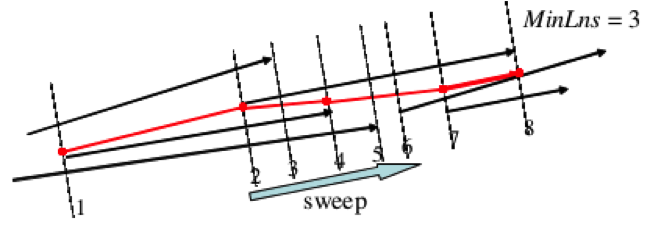
\includegraphics[scale=0.73]{traclus3}

\subsubsection{Experimental evaluation of clustering}
Seeing the plot of the clustering we can get out with some reasonable and interesting result.
The first result is the choice of the good parameter of Epsilon through a visual analysis.
The TRACLUS estimation for the player's trajectories suggests a parameter of 20. However, we started to see how the quality of cluster was affected starting with a very low parameter going ahead with 5, 10 and 15. We experimented that aspect on a striker after 4 minutes of match.

\begin{figure}
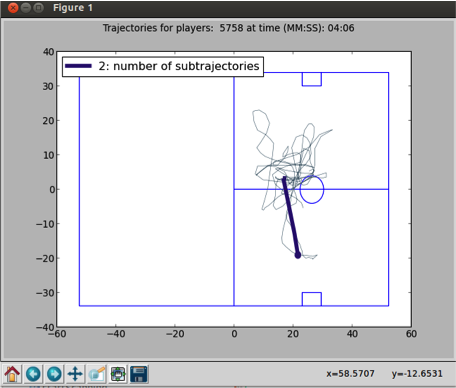
\includegraphics{experimental1}
\caption{Striker after 4 minutes with a parameter of 1 (the cluster is represented by the bold line,  instead with the thin line is represented the complete trajectory)}
\end{figure}

\begin{figure}
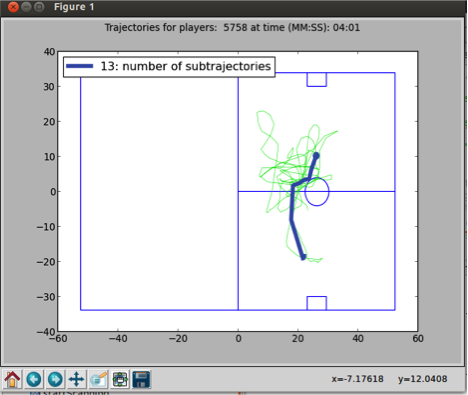
\includegraphics{experimental2}
\caption{Striker after 4 minutes with a parameter of five}
\end{figure}

\begin{figure}
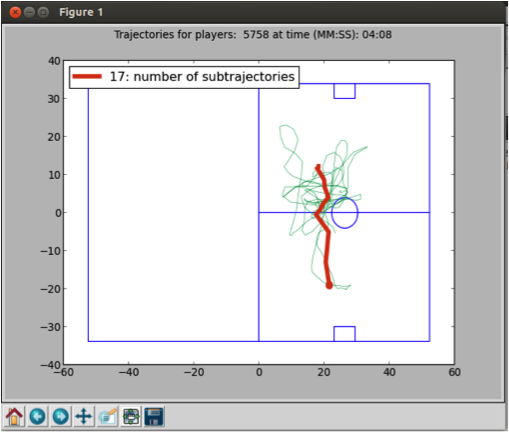
\includegraphics{experimental3}
\caption{Striker after 4 minutes with a parameter of 10}
\end{figure}

\begin{figure}
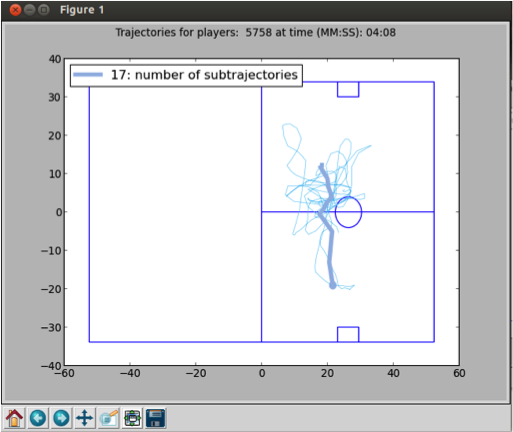
\includegraphics{experimental4}
\caption{Striker after 4 minutes with a parameter of 15}
\end{figure}

\begin{figure}
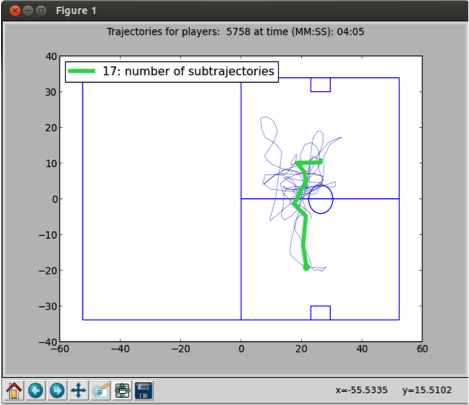
\includegraphics{experimental5}
\caption{Striker after 4 minutes with a parameter of 20}
\end{figure}

From a rapid visual investigation we can say that from 10 to 20 the quality of clustering does not change significantly and we feel free to assume that 10 for the football movement is a reasonable parameter where to around. Of course having only a dataset for one match we cannot confront with other matches. This suggests a cue for a future work that could be based on the analysis of several different matches to understand the nature of the movement.  


We also tried to discover the common trajectories of two players. For example we compared players belonging to the same team with same roles (striker) or totally different positions (striker and defender).


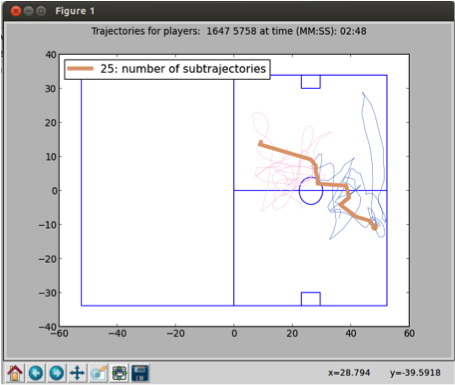
\includegraphics{experimental6}

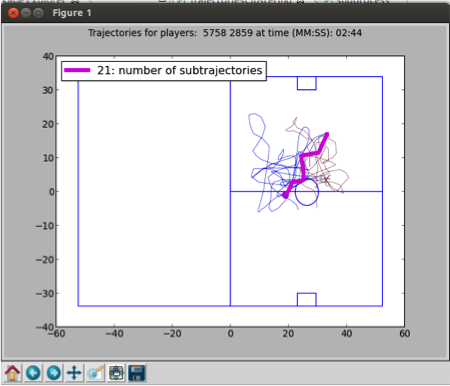
\includegraphics{experimental7}

What we can see here is that a cluster with a short representative line means that the similar trajectories are very close and the movement happen in almost the same position of the field meaning the similarity is high based on the role and the characteristic we want to study in a player. A long representative line means that the similar trajectory happen in far portions of field.  The last experiment we conducted is about the ball movement. From our analysis we can see how we understand, from the clustering, where the play with the ball is mostly developed.


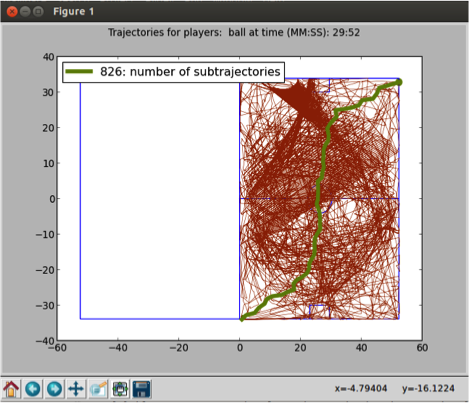
\includegraphics{experimental8}

\subsection{Speed performance analysis}
Having a real time data provided by the sensor with an high frequency one interesting problem we can solve easily is the computing of the speed performance of the player with a very little error. We found interesting know some simple but meaningful statistic as the real-time speed average, the real-time km ran for each player and the real-time performance quantified by expressiveness value as:  (stop $<=$ 1km/h , trot $<=$  11 km/h,  low $<=$ 14 km/h , medium $<=$ 17 km/h,  high $<=$ 24 km/h, sprint $>$ 24 km/h) but we found also interesting discovery some parameter coming from the comparison between the players. 

One statistic value very expressive to understand the difference in terms of running performance is the variance of the speed. Unfortunately, to compute the variance player’s data is needed and if the number of data recorded becomes huge (we have a recording frequency of 200 HZ) is practically impossible to maintain them in the main memory. A good news is that here we can exploit the streaming algorithm proposed in \cite{babcock2003maintaining}. In the first section of the paper, is proposed an approach to maintain the variance over a sliding window with a space lower bound of $\Omega( 1/e* log N *(log N + log R))$ bits for maintaining the sum (with error at most $e$) , where N is the sliding window size and each data value is at most R. (Assuming $R = poly(N)$).

\subsubsection{The streaming algorithm for the variance}
To compute an estimate of the variance with relative error at most e (with e in the range $(0, \ldots, 1)$. The elements in the data stream are partitioned into buckets by the algorithm. For each bucket $B_i$ , besides maintaining the timestamp ti of the most recent data element in that bucket, the algorithm maintains the following summary information: the number of elements in the bucket ($n_i$), the mean of the elements in the bucket ($\mu i$), and the variance of the elements in the bucket ($V_i$). The actual data elements that are assigned to a bucket are not stored. In addition to the buckets maintained by the algorithm, another set of suffix buckets, denoted $B_1 \cdots B_j$ , are stored and they represent suffixes of the data stream. Bucket $B_i\star$ represents all elements in the data stream that arrived after the elements of bucket $B_i$ , that is, $B_m\star = \bigcup _{l=1}^{i-1}B_l$. Except for the bucket $B_m\star$ , which represents all points arriving after the oldest non-expired bucket, these suffix buckets are not maintained by the algorithm, though their statistics are calculated temporarily during the course of the algorithm.

How to compute the variance? Let $B_1 \cdots B_m$ be the set of histogram buckets at time $t$. Let $B_m$ be the oldest active bucket. It contains some active elements, including the one with timestamp N, but may also contain expired data. The algorithm maintains statistics corresponding to $B_{m\star}$, the suffix bucket containing all elements that arrived after bucket $B_m$. To this end, we use the combination rule for every new data element that arrives. Whenever the oldest bucket gets deleted, we can find the new $B_{m\star}$ by “deleting” the contribution of the new oldest active bucket ($B_m$) from the previous $B_{m\star}$, using the combination rule. 
Let $B_{m\wr}$ refer to the non-expired portion of the bucket $B_m$ , i.e., the set of elements in $B_m$ that are still active. 
Since we do not know the statistics $B_{m\wr}$, $\mu_{m\wr}$  and $V_{m\wr}$ corresponding to bucket $B_{m\wr}$, we estimate them as follows: $n_{m\wr} ^{EST}= N + 1 - t_m; \mu_{m\wr} ^{EST} = \mu m $; $V_m{\wr} ^{EST} = \frac{V_m}{2}$ 

The statistics for $B_{m\wr}$ and $B_{m\star}$ are sufficient to accurately compute the variance at the time instant t. In fact the variance is nothing but the variance corresponding to the bucket $B_{m  \wr, m\star}$ obtained by combining $B_{m\wr}$ and $B_{m\star}$. 

Therefore, by the combination rule, the actual variance ($VAR(t)$) for the current active window is given by:


$$VAR(t) = V_{m\wr} + V_{m\star} + \frac{n_{m\wr}*n_{m\star}}{n_{m\wr}+n_{m\star}} *(\mu_{m\wr} – \mu_{m\star})^2$$

Having the possibility to compute the variance of the speed with a streaming fashion we found interesting to have 2 measure of comparison. The self-comparison for each player, in other word, having at real-time the variance of the player in the last m minutes (the size of the window is decided by the user). The second measure concerning the variance of speed for the average speed of the player divided by the role (only for the movement player: defenders, mid fielders, strikers). 

\subsubsection{Results of the performance speed analysis}
At the end we have the possibility to show in real time such plots. Two examples are reported in this paper.
\begin{figure}
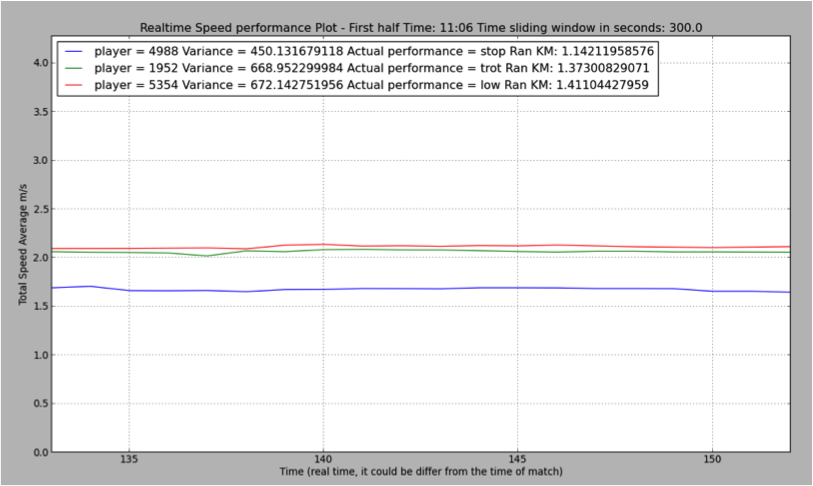
\includegraphics[scale=0.6]{fuck1}
\caption{Here we can see the variance of speed in the last 5 minutes (the size of window) respect the total average. Attached to the label of the plot we can see the instantaneous statistic of the performance all of them computed in O(1) thanks to the data come from the sensor.}
\end{figure}

\begin{figure}
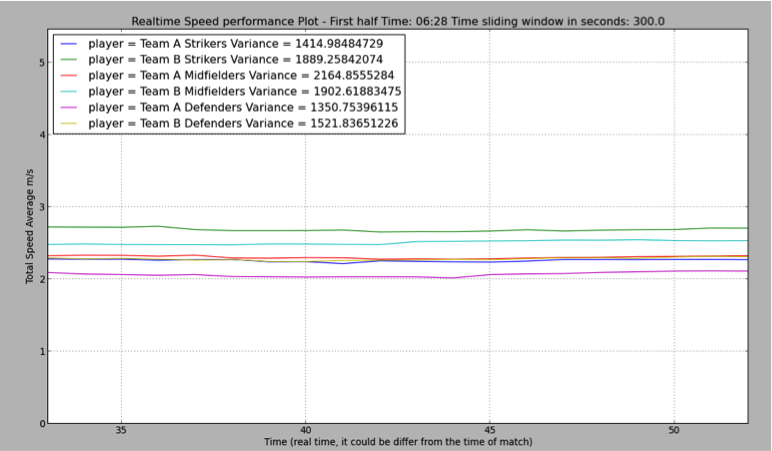
\includegraphics[scale=0.6]{fuck2}
\caption{Here instead we can see the aggregate statistic for the player divided by role.}
\end{figure}

\section{Future works}

\begin{description}
  \item[I/O dependence] Our code is high I/O depedent so, in order to speed up the whole operations it would be interesting to use a scalable framework as Map/Reduce and split the operations between many machines.
  \item[Incremental trajectories] It would be interesting to apply an incremental trajectory clustering \cite{li2010incremental}
  \item[Scalability] We could focus a future work comparing the possible different results obtained by applying this framework to different matches.
\end{description}

\section{Conclusions}
In this work, we have proposed a new approach to extract hidden informations from a football match dataset yield by an innovative sensor system provided by Fraunhofer. This system in an alternative to video-motion analysis which provides reliable informations and it is a possible new fashon which can be adopted from different clubs and FIFA organization. 

The intense competitive schedules of elite soccer clubs require data to be available usually within 24-36 hours post-match \cite{Figueroa2006122} and our system provides all the qualitative data in real-time. Moreover the interesting fact is the scalable nature of our approaches. According to the needs of the football professionals we can analyze other several factor exploiting the techniques coming from the Massive Data Analytics research field with optimal usage of the computing resource (e.g.. the memory usage with the increasing of the data). 

When Bill James and the SABR-metricians were making their contributions to baseball, they worked with public data. Now that sport analytics seems to be mainstream, we hope that a new soccer big data era is coming. For this reason we provided a framework of tools which permits the coaches to base their new strategies not only on their intuitions and judgments but also on comprensive (and maybe not human-eye-visible) statistics. Moreover we made it free and public at this URL \url{http://git.io/ms-8XA}.

%\end{document}  % This is where a 'short' article might terminate


%
% The following two commands are all you need in the
% initial runs of your .tex file to
% produce the bibliography for the citations in your paper.
\bibliographystyle{abbrv}
\bibliography{sigproc}  % sigproc.bib is the name of the Bibliography in this case
% You must have a proper ".bib" file
%  and remember to run:
% latex bibtex latex latex
% to resolve all references
%
% ACM needs 'a single self-contained file'!
%
%APPENDICES are optional
\balancecolumns

% This next section command marks the start of
% Appendix B, and does not continue the present hierarchy


% That's all folks!
\end{document}
